\lohead{Florian Harrer}

\chapter{Java-Programm}
\label{sec:java-programm}

\section{Anforderungen}
\subsection{Programm}
Die Hauptaufgabe des Programms ist es dem Benutzer eine Möglichkeit zum Steuern der Katzenfütterungsanlage zu Verfügung zu stellen. Weiters soll das Programm die Motoren steuern und die Sensoren in der Anlage auswerten können. Für diese Aufgabe sollen die IO-Pins am Raspberry verwendet werden.
\subsection{Design - Benutzerinterface}
Das Design der GUI-Fenster soll einfach und übersichtlich gestaltet werden. Auf der Hauptseite, also der Seite die immer zu sehen ist, sollen Informationen dargestellt werden, die dem Benutzer einen schnellen Überblick über den Zustand der Anlage geben. Alle anderen nicht direkt ersichtlichen Funktionen sollen über sinnvoll benamte Menüpunkte erreichbar sein.
Der Benutzer soll mit Hilfe eines kleinen Touchdisplays die Möglichkeit haben die Anlage zu steuern. Deswegen muss darauf geachtet werden, dass alle GUI-Fenster sinnvoll per Touch-Gesten verwenbar sind.
\subsection{Externe Steuerung}
Da die Katzenfütterungsanlage die Katze füttern soll, wenn die Familie der Katze auf Urlaub ist, sollte die Anlage auch über das Internet erreichbar sein. Dafür gibt es die Möglichkeit einen Benutzer auf der Anlage anzulegen mit welchem man anschließend über eine Webseite auf die Anlage zugreifen kann. Weiters soll das Java Programm (Server) mit der Web-Applikation (Client) kommunizieren, also Daten austauschen, können.

\newpage

\section{Voruntersuchung}
\subsection{Wieso Java und nicht C?}
Zu Beginn musste entschieden werden mit welcher Programmiersprache gearbeitet werden soll. Zur Auswahl standen Java und C.
Vorteile von C:
\begin{itemize}
\item[1] Echtzeitfähige Steuerung der Motoren und Senosren
\item[2] Hardwarenahe Programmierung für die Pins
\end{itemize}
Vorteile von Java:
\begin{itemize}
\item[1] Erstellen einer GUI ist einfacher
\item[2] Implementieren eines Servers ist einfacher
\end{itemize}

Nach dem Gegenüberstellen der Vorteile wurde Java als Programmiersprache gewählt.

\subsection{Wieso das Raspberry Pi 3 Model B?}
Schon zu Beginn der Diplomarbeit war klar, dass mit deinem Raspberry gearbeitet werden soll. Nun musste entschieden werden welches Model verwendet werden soll. Wir haben das Raspberry Pi 3 Model B aufgrund folgender technischer Daten gewählt:
\begin{itemize}
\item[1] Rechenleistung
\item[2] Anzahl der GPIO-Pins
\item[3] WLAN-Fähigkeit
\end{itemize}

\subsection{Auswahl eines Touchdisplays}
Das Display muss folgendet Anforderungen erfüllen:
\begin{itemize}
\item[1] Es muss ein Touchscreen-Display sein
\item[2] Es muss einfach an das Raspberry anschließbar sein
\item[3] Es sollte nicht zu teuer sein
\end{itemize}

Aufgrund dieser Anforderungen wurde das Touchdisplay von Raspberry gewählt.

\subsection{Wieso pi4j?}
Da Java als Programmiersprache gewählt wurde, musste eine Möglichkeit die GPIO-Pins anzusteuern gefunden werden.
Da bei der Recherche außer pi4j Java kaum etwas gefunden wurde, wurde pi4j gewählt. Weiters vorteilhaft ist, dass das Ansteuern der Pins via Code nicht sehr kopliziert ist. 

\subsection{Wieso Mongodb?}
Eine Datenbank wurde gewählt, weil es gegebüber des Speichers der Daten in eine Datei mehrere Vorteile aufweist. 
\subsubsection{Vorteil gegenüber Daten in Datei speichern}
Vorteile einer Datenbank:
\begin{itemize}
\item[1] Keine Probleme mit Pfaden
\item[2] Daten sind alle in einem Punkt gespeichert und nicht im System verteilt
\item[3] Der benötigte Code für die Datenbank macht das Programm übersichtlicher
\end{itemize}
\subsubsection{Vergleich mit anderen Datenbanken}
Vorteile von Mongodb gegenüber anderen Datenbanken (zB mySQL):
\begin{itemize}
\item[1] Mongodb ist schemenlos (Daten benötigen keine bestimmte Struktur)
\item[2] Mongodb ist kostenfrei
\end{itemize}

\subsection{Kommunikation mit der Web-Applikation}
Der Server mit dem die Web-Applikation kommunizieren kann, wird aufgrund der gewählten Programmiersprache, in Java geschrieben. Der Server wird im Hintergrund aktiv sein und auf Anfragen der Web-Applikation warten. Je nach Anfrage wird der Server Daten zurück senden oder Methoden im Programm aufrufen. Die Daten, die bei der Kommunikation ausgetauscht werden, haben den Datentyp JSON.

\newpage

\section{Umsetzung}
Bei der Umsetzung, also beim Schreiben des Programms, wurde wie folgt vorgegangen. Zuerst wurden alle GUI-Fenster per Hand grob designed. Anschließend wurden diese im Netbeans als JFrame Form erstellt. Genaueres über die GUI-Fenster folgt uner Punkt 2.3.4. Danach wurden grundlegende Funktionen die das Programm zu erfüllen hat implementiert. Weiters wurden noch: Mongodb, pi4j, der Server und der ErrorAndWarningHandler als Singleton implementiert. 
\\ \\ 
Nun folgen ausführlichere Beschreibungen über die oben angeführten Klassen.

\subsection{Mongodb}
\subsubsection{Allgemeines}
Mongodb is ein schemenlose Datenbank. Schemenlos bedeuted, dass die Daten keine besondere Formatierung brauchen um gespeichert zu werden. Zusätzlich wird jedem gespeichertem Datensatz automatisch ein einmaliger Indentifikator gegeben. Weiters ist es kostenfrei und man benötigt keine Lizenzen.
\\
Bei einer schemenbehafteten Datenbank werden die Daten in Reihen und Spalten gegliedert. Um eine solche Datenbank effizient nutzen zu können wird auch ein einmaliger Identifikator.
\\ \\ 
In Mongodb sind Zeilen Collections und Spalten Documents. 
\\ \\
Die Datenbank kann in der Konsole mit dem Befehl \textbf{mongod} gestartet werden. In unserem konkreten Fall am Raspberry startet die Datenbank beim Starten des Raspberry automatisch. Weiters kann in der Konsole mit dem Befehl \textbf{mongo}, sofern die Datenbank gestartet ist, die Mongo-Shell geöffnet werden. In der Shell können alle angelegten Datebanken verwaltet werden. Unter verwalten wird das Ändern, Hinzufügen und Löschen von Daten verstanden. Es können auch neue Datenbanken angelegt oder alte Datenbanken gelöscht werden. 
\\ Befehle:
\begin{itemize}
\item[•] \textbf{show dbs} ... zeigt alle angelegten Datenbanken an
\item[•] \textbf{show collections} ... zeigt alle collections in einer Datebank
\item[•] \textbf{use} ... verwenden einer Datenbank, falls die Datenbank noch nicht existiert wird sie neu erstellt 
\\     (Beispiel: use <Datenbankname>)
\item[•] \textbf{drop()} ... löschen einer Datenbank
\\     (Beispiel: <Datenbankname>.drop() )
\item[•] \textbf{find()} ... suchen nach bestimmten Daten 
\\     (Beispiel: db.data.find() )
\item[•] \textbf{count()} ... zählt die Dokumente in einer Collection
\\     (Beispiel: db.<Collectionname>.count() )
\item[•] \textbf{insert()} ... hinzufügen eines Dokumentes
\\     (Beispiel: db.data.insert(\{"time1":"13:30"\})
\item[•] \textbf{updateOne()} ... updaten von Daten
\\     (Beispiel: db.data.updateOne(<DokumentID>, <Daten>) )
\item[•] \textbf{deleteOne()} ... löschen eins Dokumentes
\\     (Beispiel: db.data.deleteOne(<DokumentID>) )

\end{itemize}

\subsubsection{Datenbankmanagementsystem DBS}
Ein Datenbankmanagementsystem verwaltet eine oder mehrere Datenbanken. Mehrer Datenbanken werden dabei benötigt, wenn mehrere Anwenugen oder Programme jeweils eine eigene Datenbank brauchen. Ein Beispiel für ein DBS ist Mongodb.

\subsubsection{Singleton}
Der Datenbankzugriff wurde in einem Singleton implementiert. Dadurch wird nur ein Objekt der Datenbank erzeugt. Das bedeutet, dass nur von dieser Klasse aus auf die Datenbank zugegriffen wird und nur eine Verbindung geöffnet wird.
\\ Ein weiterer Vorteil davon ist, dass wenn einmal eine andere Datenbank verwendet werden sollte, nur diese eine Klasse geändert werden muss, weil nur in dieser Klasse der Code für die spezifische Datenbank enthalten ist.

\subsubsection{Code Beispiele}
Da am Raspberry die neueste Version von Mongodb nicht funktioniert, wird die Version 2.14.2 verwendet. Weitere Details zu diesem Thema sind unter Punkt 2.4.1 zu finden.
\\ Aus diesem Grund sind auch die Methoden, die als Beispiele angeführt sind, von der älteren Version. 
\\ \\ 
Als erstes muss eine Verbindung mit der Datenbank aufgebaut werden. Falls die Datenbank noch nicht existiert wird sie automatisch erstellt.
Dies ist in Java mit folgenden Methoden möglich:
\begin{lstlisting}[style=JavaStyle, caption=Mit Mongodb verbinden]
	MongoClient mongodb = new MongoClient();
	DB database = mongodb.getDB("<Datenbankname>");
\end{lstlisting}

Danach muss die Collection, in der gearbeitet werden soll, ausgewählt werden. Falls die Collection noch nicht existiert wird sie automatisch erstellt. Das ist mit der folgenden Methode möglich:
\begin{lstlisting}[style=JavaStyle, caption=Collection auswählen]
	DBCollection coll = database.getCollection("<Collectionname>");
\end{lstlisting}
Anschließend kann mit der Datenbank gearbeitet werden. 
\begin{itemize}
\item[•] Die Dokumente in einer Collection zähle1n:
\begin{lstlisting}[style=JavaStyle, caption=Anzahl der Collections zählen]
	<Collectionname>.count();
\end{lstlisting}
\item[•] Ein Dokument aus der Datenbank lesen:
\begin{lstlisting}[style=JavaStyle, caption=Nach Dokument suchen]
	DBObject document = <Collectionname>.find(<Identifikator>).next();
\end{lstlisting}
\item[•] Ein Dokument zu einer Collection hinzufügen:
\begin{lstlisting}[style=JavaStyle, caption=Ein Dokument hinzufügen]
	<Collectionname>.insert(document);
\end{lstlisting}	
\item[•] Ein Dokument in einer Collection updaten:
\begin{lstlisting}[style=JavaStyle, caption=Ein Dokument updaten]
	<Collectionname>.update(<Identifikator>, document);
\end{lstlisting}
\end{itemize}

Bevor das Java Programm beendet wird sollte die Verbindung zur Datenbank wie folgt getrennt werden: 
\begin{lstlisting}[style=JavaStyle, caption=Verbindung zur Datenbank trennen]
	mongodb.close();
\end{lstlisting}

Ein konkretes Beispiel des Codes aus dem Programm für die Katzenfütterungsanlage sieht so aus:
\begin{lstlisting}[style=JavaStyle, caption=Konkretes Beispiel: Dokument suchen]
	DBObject document = collUser.find(
			new BasicDBObject("identifier", "User")).next();
\end{lstlisting}
Diese Zeile Code sucht in der Collection \textbf{collUser} nach dem Dokument mit dem Identifikator \textbf{new BasicDBObject(\grqq{}identifier\grqq{}, \grqq{}User\grqq{})}. Das gefundene Dokument wird dann der Varibale \textbf{document} zugewiesen. 


\subsection{pi4j} \label{subsec:pi4j}
\subsubsection{Allgemeines}
Pi4j ist eine freie Software, welche Bibliotheken zur Verfügung stellt, mit denen es möglich ist, von einem Java Programm, auf die IO-Pins eines Raspberrys zuzugreifen. Dabei kann ein GPIO-Pin als In- oder Ouput definiert werden. Wenn ein Pin als Output definiert wird, kann er den State High (+5V) oder Low (0V) haben. Mit einem Input Pin, können Signale gemessen werden. Das Ergebnis der Messung ist wieder High oder Low. Weiters ist es auch möglich einem Pin einen Listener zuzuweißen. Dieser Listener wartet bis auf diesem Pin ein Event auftritt und führt dann zum Beispiel eine Methode aus. 
\\ \\
Pi4j stellt eine Verbindung von der JVM (Java Virtuaul Machine) zu dem nativen System des Raspberys her. Dadurch wird es möglich von dem Programm auf die Pins zuzugreifen. Die folgende Grafik zeigt welche Bibliotheken dazu verwendetwerden.

\begin{wrapfigure}{l}{0.5\textwidth}
\vspace{-35pt}
  \begin{center}
    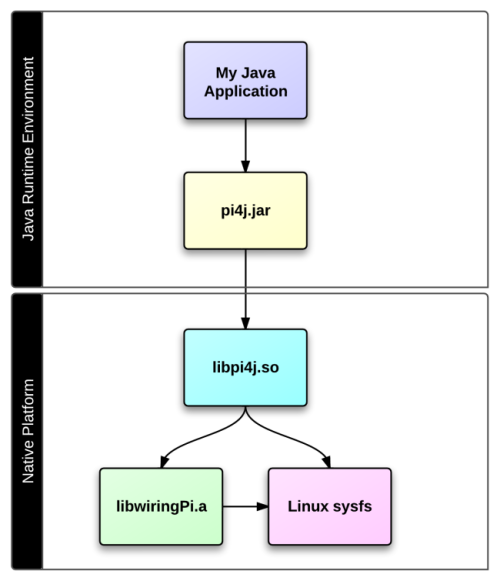
\includegraphics[width=0.45\textwidth]{Bilder/pi4j/dependencies}
  \end{center}
  \caption{Abhängigkeiten}
  \label{Magazin Vorne}
  \vspace{-170pt}
\end{wrapfigure}

Pi4j stellt eine Verbindung von der JVM (Java Virtuaul Machine) zu dem nativen System des Raspberys her. Dadurch wird es möglich von dem Programm auf die Pins zuzugreifen. Die folgende Grafik zeigt welche Bibliotheken dazu verwendetwerden.

\newpage

\subsubsection{Pin Numbering Sheme}

\begin{wrapfigure}{l}{0.5\textwidth}
\vspace{-40pt}
  \begin{center}
    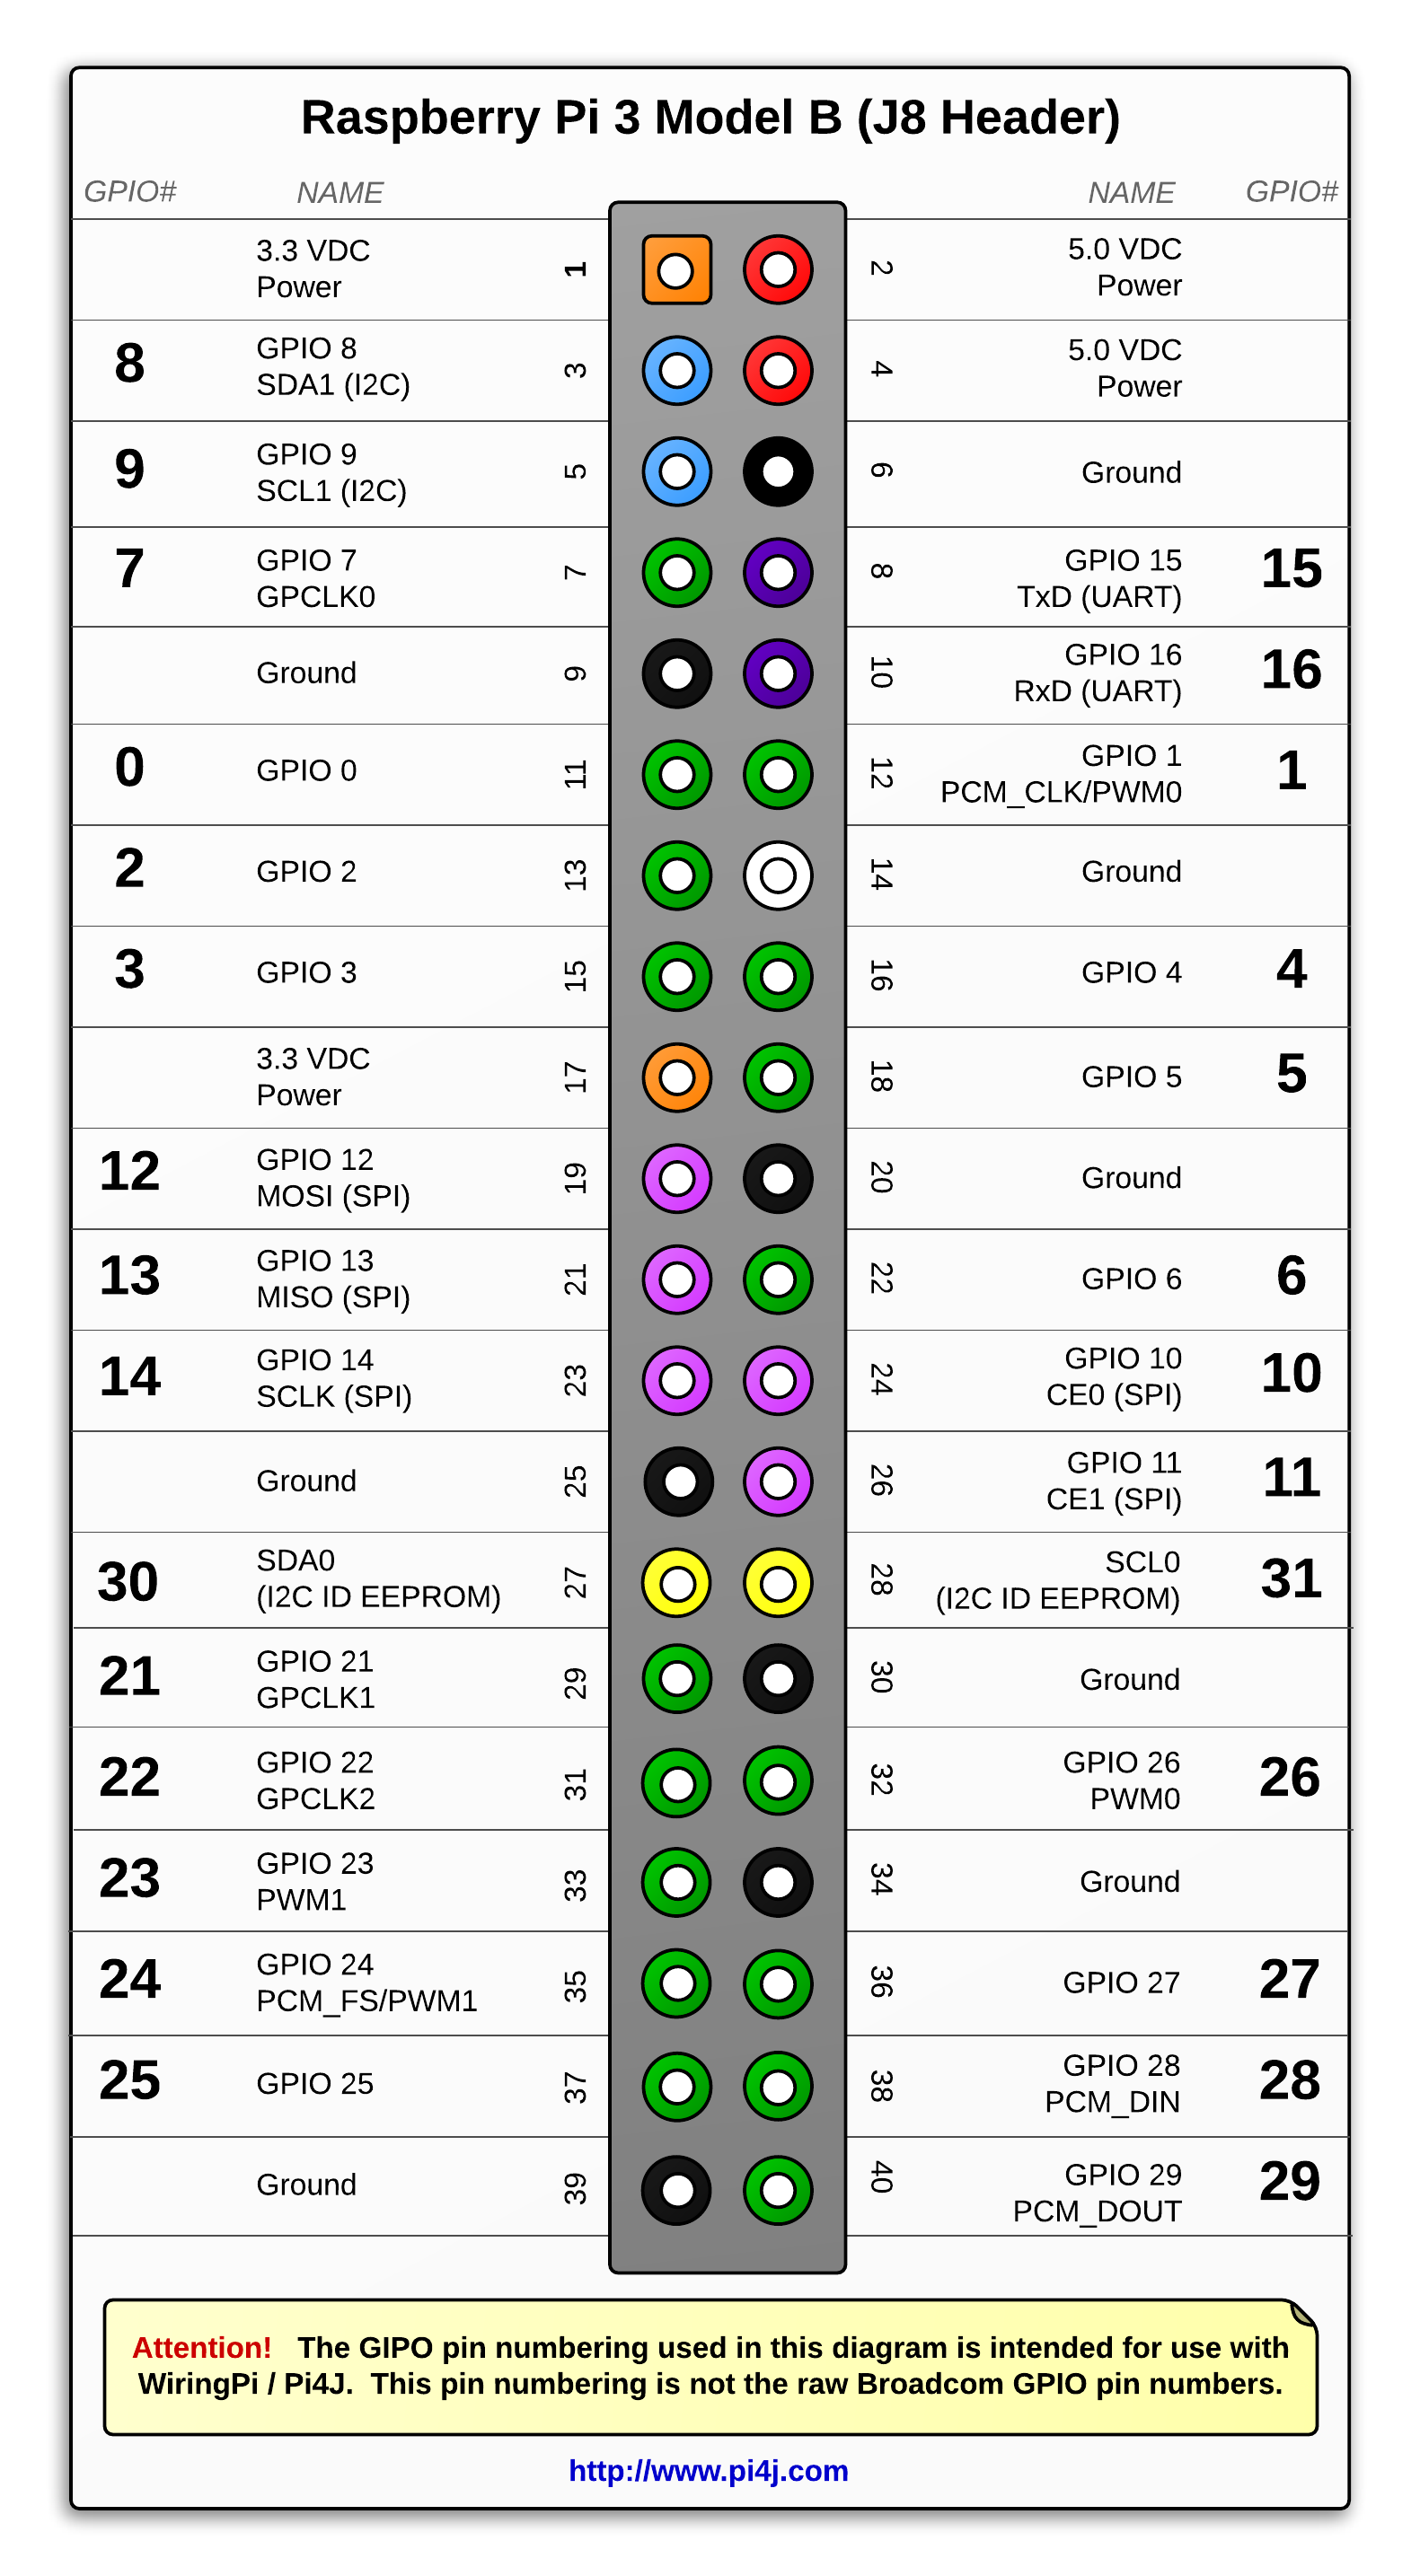
\includegraphics[width=0.50\textwidth]{Bilder/pi4j/PinNumberingSheme}
  \end{center}
  \caption{Pin Numbering Sheme}
  \label{Magazin Vorne}
  \vspace{-320pt}
\end{wrapfigure}

Am Raspberry haben einige Pins schon fest zugewiesene Funktionen, aber bei den GPIO-Pins kann der Programmierer selbst entscheiden, was der Pin sein soll.
\\ \\
In der Grafik ist zu sehen wie die Pins bei einem Raspberry Pi 3 Model B belegt sind.

\vspace{300pt}

\subsubsection{Gewählte Pin Belegung}
Zum Ansteuern der Motoren und Auswerten der Sensoren wurden nur GPIO-Pins verwendet. Die Motoren in der Anlage werden über jeweils eine H-Brücke angesteuert. Das bedeutet, dass jeder der zwei Motoren jeweils mit vier Transitoren angesteuert wird. Jeder Transitor wird von einem eigenen Pin angesteuert. Für die Sensoren wird jeweils ein Pin zum Auswerten benötigt. In Summe werden zehn GPIO-Pins benötigt. 

\newpage

Diese GPIO-Pins werden, wie folgenden Tabelle 2.1 veranschaulicht, verwendet:

\begin{table}[htb]
\centering
\begin{tabular}{|l|l|}
\hline
\textbf{Pin} & \textbf{Verwendungszweck}          \\ \hline
GPIO\_00     & Sensor Schüsselplatte              \\ \hline
GPIO\_01     & Sensor Förderband (Futtersackerl)  \\ \hline
GPIO\_02     & Motor Schüsselplatte: Transistor 1 \\ \hline
GPIO\_03     & Motor Schüsselplatte: Transistor 2 \\ \hline
GPIO\_04     & Motor Schüsselplatte: Transistor 3 \\ \hline
GPIO\_05     & Motor Schüsselplatte: Transistor 4 \\ \hline
GPIO\_06     & Motor Förderband: Transistor 1     \\ \hline
GPIO\_10     & Motor Förderband: Transistor 2     \\ \hline
GPIO\_08     & Motor Förderband: Transistor 3     \\ \hline
GPIO\_09     & Motor Förderband: Transistor 4     \\ \hline
\end{tabular}
\caption{Belegung der GPIO-Pins}
\label{Pinbelegung}
\end{table}

Wenn einer der beiden Sensoren betätigt wird, liefert dieser das Signal High (+5V). Wenn der Sensor nicht betätigt ist liefert dieser Low (0V). 
\\ Um einen Motor einzuschalten müssen jeweils zwei diagonal zueinander liegende Transitoren aktiviert werden. Der Motor dreht sich im Uhrzeigersinn, GPIO-Pins von Transistor 1 und Transistor 4 High sind. Gleichzeitig muss sicher gestellt werden, dass die GPIO-Pins der Transistoren 2 und 3 Low sind. Wenn das nicht sichergestellt ist kann es zu einem Kurzschluss zwischen der Spannungsversorgung und GND kommen. Um den Motor gegen den Uhrzeigersinn zu drehen müssen die GPIO-Pins der Transistoren 2 und 3 auf High sein. 

\subsubsection{Singleton}
Die benötigten Methoden von pi4j wurden in einem Singleton implementiert. Es musste ein Singleton verwendet werden, weil der benötigte Controller für die Pins nur einmal erzeugt werden kann. Wenn der Controller trotzdem öfters erzeugt wird, wird  ein Error geworfen. Der Singleton wird nun dazu verwendet, dass auf die Pins von unterschiedlichen Klassen zugegriffen werden kann. Der Zugriff von mehreren Klassen ist ohne einen Singleton programmiertechnisch nicht lösbar.

\subsubsection{Code Beispiele}
Um mit den GPIO-Pins arbeiten zu können muss zu Beginn ein Controller erstellt werden. Dies ist wie folgt möglich:
\begin{lstlisting}[style=JavaStyle, caption=GPIO-Controller erstellen]
	GpioController controller = GpioFactory.getInstance();
\end{lstlisting}
Wenn der Controller erstellt ist kann auf die Pins, mit denen gearbeitet werden soll, zugegriffen werden. Bei einem Pin kann auch eine \textbf{ShutDownOption} angeben werden. Diese gibt an in welchen Zustand der Pin vor dem Herunterfahren gesetzt wird. Dieser Zugriff erfolgt wie folgt: 
\begin{itemize}
\item[•] Zugreigen auf einen Pin als digitalen Input-Pin:
\begin{lstlisting}[style=JavaStyle, caption=Zugriff auf einen Pin als Inpput]
	GpioPinDigitalInput pin = controller.provisionDigitalInputPin(
		RaspiPin.GPIO_00, PinPullResistance.PULL_DOWN);
	pin.setShutdownOptions(true);
\end{lstlisting}
\item[•] Zugreigen auf einen Pin als digitalen Output-Pin:
\begin{lstlisting}[style=JavaStyle, caption=Zugriff auf einen Pin als Output]
	GpioPinDigitalOutput pin = controller.provisionDigitalOutputPin(
		RaspiPin.GPIO_02, PinState.LOW);
	pin.setShutdownOptions(true, PinState.LOW);
\end{lstlisting}
\end{itemize}
Wenn das erledigt ist kann mit dem Pin gearbeitet werden. Dies kann wie in den folgenden Beispielen erfolgen:
\begin{itemize}
\item[•] Zustand eines Input-Pins auswerten: 
\begin{lstlisting}[style=JavaStyle, caption=Pinzustand abfragen]
	pin.getState()
\end{lstlisting}
Diese Methode liefert den Zustand des Pins zurück. Dieser kann High oder Low sein.
\item[•] Zustand eines Output-Pins setzen:
\begin{lstlisting}[style=JavaStyle, caption=Pinzustand verändern]
	pin.low();	
	pin.high();
\end{lstlisting}
Mit \textbf{pin.low()} kann der Zustand eines Pins auf Low (0V) und mit \textbf{pin.high()} auf High (+5V) gesetzt werden. 
\end{itemize}

Vor dem Beenden des Java Programmes sollte der Controller wie folgt heruntergefahren werden:
\begin{lstlisting}[style=JavaStyle, caption=Controller herunterfahren]
	controller.shutdown();
\end{lstlisting}

\newpage

\subsection{Server-Client-Kommunikation}
\subsubsection{Server}
Der Server wird beim Starten des Java Programmes in einem eigenen Thread gestartet. In diesem Thread wartet der Server bis ein Client versucht Kontakt mit ihm aufzunehmen. Wenn die Verbindung akzeptiert wird, wird ein neuer Thread geöffnet in dem die Kommunikation mit diesem Client abläuft. Sobald die Kommunikation beendet ist wird der Thread wieder geschlossen. 
\\ Der Server wurde auch als Singleton implementiert damit von mehreren Klassen ausgehend auf ihn zugegriffen werden kann.

\subsubsection{Übertragungsprotokoll}
Im Übertragungsprotokoll wird festgelegt wie die Kommunikation zwischen Server und Client abläuft. Hier wird festgelegt was ein gültige Request (Anfrage) ist und wie die Response (Antwort) auf den jeweiligen Request aussieht. 
\\ \\
Wenn der Request des Clients mit einem \textbf{GET} beginnt, bedeutet dass, das der Client Daten vom Server fordert. Beginnt der Request mit einem \textbf{PUT}, bedeutet dass, das der Client dem Server Daten schicken will.
\\ Nach jedem \textbf{GET} oder \textbf{PUT} folgt ein URL der angibt, welche Daten der Client fordert oder welche Daten der Client dem Server schicken will.
\\ \\
Die folgende Tabelle zeigt alle gültigen Requests und die jeweilige Response darauf:

\begin{table}[htb]
\centering
\begin{tabular}{|l|l|p{300pt}|}
\hline
\multicolumn{2}{|c|}{\textbf{Request}}                                    & \multicolumn{1}{c|}{\multirow{2}{*}{\textbf{Response}}}                                          \\ \cline{1-2}
\multicolumn{1}{|c|}{\textbf{Aktion}} & \multicolumn{1}{c|}{\textbf{URL}} & \multicolumn{1}{c|}{}                                                                            \\ \hline
GET                                   & /errors\_warnings                 & Der Server schickt dem Client die aktuell anzuzeigenden Errors und Warnungen in einer Json-Array \\ \hline
PUT                                   & /ChangeMachineState               & Der Server ruft eine Methode auf um den Maschinenzustand zu ändern                               \\ \hline
\end{tabular}
\caption{Übertragungsprotokoll}
\label{Übertragungsprotokoll}
\end{table}

\newpage

\subsubsection{Response-GET}
Wenn der Server einen Request mit dem Beginn \textbf{GET} bekommt, muss er dem Client die Daten schicken. 
\\ Bei der Katzenfütterungsanlage werden dem Client vom Server die ganzen auftretenten Errors und Warnungen geschickt. Die Errors und Warnungen werdem dem Client als Json-Array geschickt. Diese Json-Array wird in der Klasse, welche alle Errors and Warnungen verarbeitet, erstellt. Die Json-Array ist unter Punkt \ref{subsubsec:Array} dargestellt. 

\subsubsection{Response-PUT}
Wenn der Server einen Request mit dem Beginn \textbf{PUT} bekommt, muss er Daten vom Client entgegen nehmen.
\\ Bei der Katzenfütterungsanlage bekommt der Server die Daten nicht direkt. Da der Maschinenzustand nur \textbf{Ein} oder \textbf{Aus} sein kann, wird dieser nicht übermittelt. Stattdessen wird, wenn der Maschinenzustand geändert wird, die Methode \textbf{machineStateChanger()} aufgerufen, welche ihn ändert. Diese Methode aktualisiert auch die GUI-Elemente am Raspberry, abhägig vom Maschinenzustand. 

\subsubsection{Verarbeiten des Requests}
Um den Request zu verarbeiten wurde die Klasse \textbf{ConnectionThread} geschrieben. Der Request wird wie folgt verarbeitet:
\begin{itemize}
\item[1] Der Request wird eingelsen.
\item[2] Danach wird überprüft ob der Request "GET\grqq{} oder "PUT\grqq{} enthält. Wenn keine dieser beiden Funktionen enthalen ist, wird eine Fehlermeldung gesendet.
\item[3] Wenn dies überprüft wurde und kein Fehler aufgetreten ist, wird der URL überprüft. Im URL wird dem Server mitgeteil was er machen soll. Der Inhalt des URL ist ein String und wird im Übertragungsprotokoll festgelegt.
\end{itemize}

\subsection{Errors und Warnungsverarbeitung}
\subsubsection{Allgemeines}
Der Benutzer der Katzenfütterungsanlage muss über Fehler, die während des Programmablaufs auftreten, informiert werden. 
\\ Dazu dient die \textbf{ErrorAndWarningHandler\_Singleton} Klasse. In dieser Klasse wird beim Auftreten eines Fehlers eine Boolean Variable auf \textbf{true} gesetzt. Beim Erstellen der Liste, die die Errors und Warnungen enthält, werden die jeweiligen Boolean-Variablen abgefragt. Wenn die Boolean-Variable \textbf{true} ist, wird der Error oder die Warnung hinzugefügt. 

\newpage

\subsubsection{Errors und Warnungen aktivieren/deaktivieren}
Um die Boolean-Variable, die die Errors and Warnungen aktiviert, auf true zu setzen, muss die jeweils zum Error oder zur Warnung gehörende Methode aufgerufen werden. Diese Methode kann wie folgt aussehen:
\begin{lstlisting}[style=JavaStyle, caption=Error setzen]
public void setFeedingHasFailedError (Boolean errorOn, String errorTime)
    {
        error_hasFeedingFailed = errorOn;
        failedFeedingTime = errorTime;
    }
\end{lstlisting}
In diesem konkreten Beispiel wird der Error, der dem Benutzer mitteilt, dass eine Fütterung fehlgeschlagen hat, aktiviert. Mit dem Parameter \textbf{errorOn} kann bestimmt werden, ob der Error aktiv oder inaktiv sein soll. Wenn der Parameter \textbf{true} ist, ist der Error aktiv. Daraus folgt, dass der Error inaktiv ist, wenn \textbf{errorOn = false} ist. 
\\ Mit dem zweiten Parameter \textbf{errorTime} wird die Zeit übergeben, zu der die Fütterung fehlgeschlagen ist. Diese Zeit wird dann in der Errormeldung ausgegeben. 

\subsubsection{Json-Array} \label{subsubsec:Array}
Diese Klasse stellt auch die Json-Array zur Verfügung, welche dann dem Client (Web-Applikation) geschickt wird. 

Die JsonArray sieht wie folgt aus:

\begin{lstlisting}[language=json,firstnumber=1, caption=Json-Objekt mit Errors und Warnungen]
{ 
	"Errors": 
	[ 
		{"message" : "Error1", "hidden" : false}, 
		{"message" : "Error2", "hidden" : false} 
	] 
	"Warnings": 
	[ 
		{"message" : "Warning1", "hidden" : false}, 
		{"message" : "Warning2", "hidden" : false} 
	] 
} 
\end{lstlisting}

\newpage

\subsubsection{Listenmodel}
Die Zeile, in der die Klasse für das Listenmodel angelegt wird, sieht wie folgt aus:
\begin{lstlisting}[style=JavaStyle, caption=Listenmodel-Klasse erstellen]
	public class ErrorAndWarningModel extends AbstractListModel
\end{lstlisting}
Nach dem Klassennamen muss \textbf{extends AbstractListModel} hinzugefügt werden. Dies bedeutet, dass das erstellte Listemodel eine Vererbung von \textbf{AbstractListModel} ist.
\\ \\
Das Listenmodel wird wie folgt angelegt:
\begin{lstlisting}[style=JavaStyle, caption=Liste erstellen im Model]
	private final List<String> errorAndWarning;
\end{lstlisting}
Damit ist nun festgelegt, dass die Elemente in der Liste Strings sind. 

\subsubsection{Liste}
Eine Liste in Java wird dazu verwendet, um mehrere Daten in einem Objekt zu speichern. Die Liste kann wie folgt erstellt werden:
\begin{lstlisting}[style=JavaStyle, caption=Liste erstellen]
	List<String> list = new ArrayList();
\end{lstlisting}
Das Objekt der Liste verfügt über eigene Methoden. 
\begin{itemize}
\item[•] Anzahl der Elemente in der Liste zählen: 
\begin{lstlisting}[style=JavaStyle, caption=Anzahl der Elemente abfragen]
	list.size();
\end{lstlisting}
\item[•] Hinzufügen eines Elementes:
\begin{lstlisting}[style=JavaStyle, caption=Element hinzufügen]
	list.add("Das ist ein Element!");
\end{lstlisting}
\item[•] Leeren der Liste (Löschen aller Elemente)
\begin{lstlisting}[style=JavaStyle, caption=Liste leeren]
	list.clear();
\end{lstlisting}
\end{itemize}

Die Errors und Warnungen, die in der Liste gespeichert werden, werden in der GUI in einer Liste (jList) dargestellt. Siehe Kapitel \ref{subsubsec:MainWindow}. 

\subsection{SwingWorker}
Der SwingWorker in Java wird benötigt, wenn eine Anwendung mehr Zeit benötigt. Mithilfe des SwingWorkers kann diese Aktion im Hintergrund ausgeführt werden. Der Vorteil davon ist, dass die GUI verwendbar bleibt und nicht blockiert. Dafür wird dann mit Hilfe des SwingWorkers ein Hintergrund-Thread geöffnet in dem die Aktion, die mehr Zeit benötigt, abgearbeitet wird.
\\ \\ Um den SwingWorker verwenden zu können, muss die Klasse wie folgt erstellt werden:
\begin{lstlisting}[style=JavaStyle, caption=SwingWorker Klasse erstellen]
	private class Worker extends SwingWorker<Object, String> { } 
\end{lstlisting}
Im Generic steht als erstes der Rückgabewert von \textbf{done()} und als zweites der Rückgabewert von \textbf{process()}.

\subsubsection{EDT}
Im Event Dispatch Thread (EDT) wird die GUI sequentiell abgearbeitet. Dies bedeutet, dass alle Methoden ihre benötigte Zeit in Anspruch nehmen und danach die jeweils Nächste ausgeführt wird. Im Grunde wird dann ein SwingWorker verwendet, wenn die GUI für den Benutzer merklich blockiert. 

\subsubsection{TimeUnit}
Wenn ein Hintergrund-Thread mit einer \textbf{while() Schleife} implementiert ist, wiederholen sich die Methoden in der Schleife nach jedem Durchgang wieder. Wenn dies ohne ein Warten passiert, wird sehr viel Prozessorleistung benötigt. Deswegen wird ein \textbf{TimeUnit.MILLISECONDS.sleep(500);} verwendet. Mit dieser Methode wartet das Programm, an der Stelle wo die Methode aufgerufen wird, für 500 Millisekunden. Dadurch wird der Prozessor nicht so stark ausgelastet. 

\subsubsection{Methoden des SwingWorkers}
\begin{itemize}
\item[•] doInBackground()
\\ Mit \textbf{doInBackground()} kann ein neuer Hintergrund-Thread geöffnet werden. Dieser Thread läuft parallel zum EDT. Der Hintergrund-Thread wird geschlossen, wenn der Worker beendet wird oder sich der Worker selbst beendet, weil er alle Methoden abgearbeitet hat. In einem Hintergrund-Thread darf nicht auf GUI-Elemente zugegriffen werden. 
\\ Im folgenden Beispiel wird ein Hintergrund-Thread gezeigt, welcher nur durch das Beenden des Workers beendbar ist.
\begin{lstlisting}[style=JavaStyle, caption=SwingWorker doInBackground() mit while Schleife]
	    @Override
        protected Object doInBackground() throws Exception
        {
            while (!isCancelled())
            {
                timeOfDay = String.format("%1$tH:%1$tM", new
                Date(System.currentTimeMillis()));

                publish( timeOfDay);

                TimeUnit.MILLISECONDS.sleep(500);
            }
            return 1;
        }
\end{lstlisting} 
Folgender Hintergrund-Thread arbeitet die Methoden nur einmal ab und wird dann. beendet. 
\begin{lstlisting}[style=JavaStyle, caption=SwingWorker doInBackground() ohne while Schleife]
	    @Override
        protected Object doInBackground() throws Exception
        {
            timeOfDay = String.format("%1$tH:%1$tM", new 
            Date(System.currentTimeMillis()));

            publish( timeOfDay);

            TimeUnit.MILLISECONDS.sleep(500);
            return 1;
        }
\end{lstlisting} 

\item[•] done()
\\ Wenn ein Hintergrund-Thread beendet wird, wird \textbf{done()} im EDT aufgerufen. Im \textbf{done()} können dann GUI-Elemente bearbeitet werden.
\begin{lstlisting}[style=JavaStyle, caption=SwingWorker done()]
	    @Override
        protected void done()
        {
             // TODO
        }
\end{lstlisting}
\item[•] process()
\\ Wenn in einem Hintergrund-Thread \textbf{publish();} aufgerufen wird, wird im EDT \textbf{process()} aufgerufen. Hier können wieder GUI-Elemente bearbeitet werden.
\begin{lstlisting}[style=JavaStyle, caption=SwingWorker process()]
	    @Override
        protected void process(List<String> chunks)
        {
        	(timeOfDay = chunks.get((chunks.size() - 1));
            lbTimeOfDay.setText(timeOfDay);
        }
\end{lstlisting}
\item[•] cancel()
\\ Mit \textbf{cancel} kann ein Worker beendet werden. Dafür muss folgender Befehl aufgerufen werden:
\begin{lstlisting}[style=JavaStyle, caption=SwingWorker abbrechen]
	    worker.cancel();
\end{lstlisting}
Bei diesem Methodenaufruf ist \textbf{worker} die Objektvariable des Workers.
\end{itemize}

\subsection{GUI-Fenster}
Die GUI-Fenster stellen die grafische Oberfläche für den Benutzer zur Verfügung. Da ein Touchscreen-Display verwendet wird, ist es möglich alle GUI-Fenster mittels Touch-Gesten zu bedienen. 
\\ Beim Starten des Raspberrys wird das Programm automatisch gestartet. Dabei wird das MainWindow, also das Hauptfenster des Programms, als Vollbild am Display angezeigt. Somit ist es dem Benutzer nur möglich das Programm zu bedienen und nicht zur grafischen Oberfläche des Raspberrybetriebsystems zu gelangen. Genauers zum Autostart unter Kapitel \ref{subsubsec:Autostart}.

\subsubsection{Java-Programm im Autostart}\label{subsubsec:Autostart}
Um auf einem Bitriebssstem ,das auf Linux basierendem, ein Java-Programm zu starten gibt es zwei Möglichkeiten.
\begin{itemize}
\item[1] \textbf{rc.local}
\\ Eine Möglichkeit ist die \textbf{rc.local}. Mit der \textbf{rc.local} können aber nur Programme ohne grafische Oberfläche gestartet werden. In diese muss foglender Befehl geschrieben werden: 
\\ \textbf{java -jar /home/pi/main.jar \&}.
\item[2] \textbf{autostart}
\\ Dies zweite Möglichkeit ist \textbf{autostart}. Hier ist der X-Server, welcher für eine grafische Ausgabe benötigt wird, enthalten. Somit können nun Java-Programme mit einer grafischen Oberfläche gestartet werden. Die Datei \textbf{autostart} ist unter folgendem Pfad zu finden : 
\\ \textbf{/home/<user/.config/lxsession/LXDE-<user>/autostart}. 
\\ In die Datei muss dann noch folgender Befehel eingegeben werden: 
\\ \textbf{@java -jar /home/pi/main.jar \&}.
\end{itemize} 
Bei beiden Möglichkeiten wird jeweils \textbf{main.jar} als Programm angegeben. Dies stellt im Fall eines Programms mit GUI das Hauptfenser dar. Bei der Katzenfütterungsanlage ist es das \textbf{MainWindow}.
\\ \\ Die Abkürzung \textbf{.jar} steht für "Java Archive".

\newpage

\subsubsection{MainWindow}\label{subsubsec:MainWindow}
\begin{wrapfigure}{l}{0.6\textwidth}
\vspace{-20pt}
  \begin{center}
    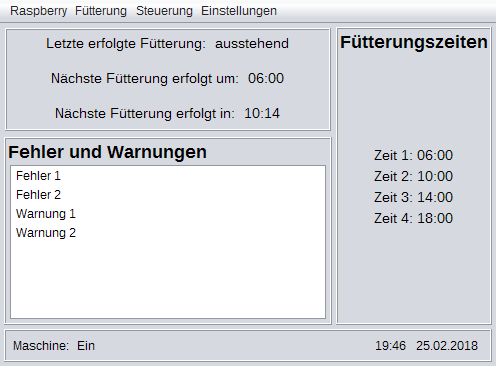
\includegraphics[width=0.60\textwidth]{Bilder/GUI/MainWindow}
  \end{center}
  \caption{MainWindow}
  \label{MainWindow}
  \vspace{-10pt}
\end{wrapfigure}
Das \textbf{MainWindow} besteht aus einer \textbf{Java JFrame Form}. In diesem Fenster wird dem Benutzer ein allgemeiner Überblick über die Anlage zur Verfügung gestellt. Somit können alle wichtigen Informationen schnell und leicht ersichtlich. Weiters ist das \textbf{MainWindow} das Hauptfenster des Programms. Über diese sind alle Dialog-,Steuerungs- und Informationsfenster erreichbar. Diese Fenster werden von Kapitel\ref{TimeManagement} bis Kapitel \ref{Update} genauer beschrieben. Das Aufrufen von anderen Fenseren ist über die Menüleiste, welche sich oben in der GUI befindet, möglich. 
\\ \\ Unter den Menüs der Menüleiste sind folgende Menüpunkte zu finden:
\begin{itemize}
\item[1] Raspberry
\begin{itemize}
\item[•] Neustarten
\item[•] Herunterfahren
\end{itemize}
\item[2] Fütterung
\begin{itemize}
\item[•] Einschalten/Ausschalten
\item[•] Fütterungszeiten verwalten
\end{itemize}
\item[3] Steuerung
\begin{itemize}
\item[•] manuelle Steuerung
\item[•] Positionsinformation
\end{itemize}
\item[4] Einstellungen
\begin{itemize}
\item[•] Update
\item[•] Benutzer anlegen
\item[•] WLAN
\item[•] Geräteinformation
\end{itemize}
\end{itemize}

\vspace{10pt}

Das \textbf{MainWindow} ist als Singleton implementiert. Somit wird ein nur Objekt des \textbf{MainWindow} erstellt. Das Singleton-Objekt wurde wie folgt erstellt:
\begin{lstlisting}[style=JavaStyle, caption=MainWindow createInstance()]
public static MainWindow createInstance()
    {
        if (instance != null)
        {
            throw new RuntimeException("intance already created");
        }

        if (!SwingUtilities.isEventDispatchThread())
        {
            throw new RuntimeException("not in EDT");
        }
        instance = new MainWindow();

        return instance;
    }
\end{lstlisting}
Diese Methode kann nur im EDT aufgerufen werden. Wenn diese Methode nicht im EDT aufgerufen wird oder das Objekt bereits besteht, wird ein jeweils eigener Error geworfen.
\\ \\ Diese Methode wird in der \textbf{main} Methode der Klasse wie folgt aufgerufen:
\begin{lstlisting}[style=JavaStyle, caption=MainWindow createInstance() Aufruf]
	java.awt.EventQueue.invokeLater(new Runnable()
        {
            @Override
            public void run()
            {
                MainWindow frame = MainWindow.createInstance();

            }
        });
\end{lstlisting}

Bis jetzt wurde der Singleton nur implementiert. Nun muss noch eine Methode implementiert werden um die \textbf{Instance} des Objekts abfragen zu können. Diese Methode sieht wie folgt aus:
\begin{lstlisting}[style=JavaStyle, caption=MainWindow.getInstance()]
public static MainWindow getInstance()
    {
        if (instance == null)
        {
            throw new RuntimeException("instance not created");
        }

        return instance;
    }
\end{lstlisting}

\vspace{10pt}

In der GUI werden je nach Maschinenstatus gewisse Funktionen blockiert. Folgende Funktionen sind blockiert, wenn die Fütterung aktiviert ist:
\begin{itemize}
\item[1] manuelle Steuerung
\item[2] Update
\end{itemize}
Das Blockieren das Funktionen wird mit folgender Methode gemacht:
\begin{lstlisting}[style=JavaStyle, caption=GUI Elemente blockieren]
private void updateGUIElements()
    {
        // control GUI elements depending on the machine state
        // update and manualControl not available while machine state = on 
        if (machineStateOn == true)
        {
            menu_update.setEnabled(false);
            menu_manualControl.setEnabled(false);
        }
        else
        {
            menu_update.setEnabled(true);
            menu_manualControl.setEnabled(true);
        }
    }
\end{lstlisting}

\newpage

\subsubsection{TimeManagement}\label{subsubsec:TimeManagement}
\begin{wrapfigure}{l}{0.65\textwidth}
\vspace{-20pt}
  \begin{center}
    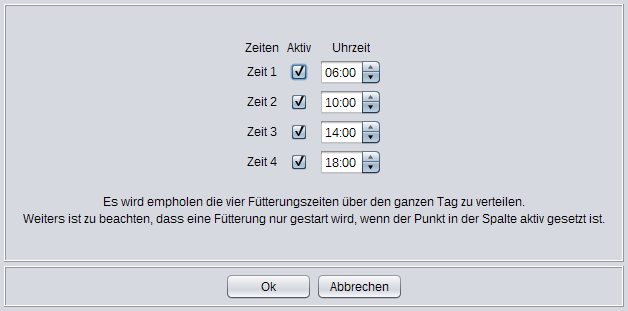
\includegraphics[width=0.65\textwidth]{Bilder/GUI/TimeManagement}
  \end{center}
  \caption{TimeManagement}
  \label{TimeManagement}
  \vspace{0pt}
\end{wrapfigure}
In der Klasse \textbf{TimeManagement} ist es dem Benutzer möglich alle Zeiten zu verwalten. Das GUI-Fenster dieser Klasse ist ein Dialogfenster. Bei Dialogfenstern ist es üblich, dass sie mit \textbf{Ok} und \textbf{Abbrechen} bedienbar sind.
\\ \\ Es können bis zu vier verschiedene Zeiten gewählt werden. Dabei müssen die Zeiten, bei Zeit 1 beginnend, aufsteigen angeordnet werden. Zusätzlich können Zeiten auch deaktiviert werden. Um eine Zeit zu deaktivieren muss das Häkchen vor der Zeit weggenommen werden.
\\ Wenn die Zeiten ausgewählt wurden, kann mit \textbf{Ok} bestätigt werden. Somit werden die Daten in das Programm übernommen und in die Datenbank gespeichert. Weiters schließt sich noch das Fenster.
\\ Falls\textbf{Abbrechen} gedrückt wird, werden die Änderungen nicht übernommen und das Fenster schließt sich.
\\ \\ Wenn das Dialogfenster im EDT aufgerufen wird, blockiert der EDT an dieser Stelle so lange, bis das Dialogfenster wieder geschlossen wird.

\newpage

Um in den Spinnern Uhrzeiten anzeigen zu lassen, müssen diese davor konfiguriert werden. Dazu muss im Designmodus der GUI Rechtsklick auf den Spinner gemacht werden. Weiters muss \textbf{Customize Code} ausgewählt werden. Anschließend öffnet sich folgendes Fenster: \\
\begin{wrapfigure}{l}{0.7\textwidth}
\vspace{-20pt}
  \begin{center}
    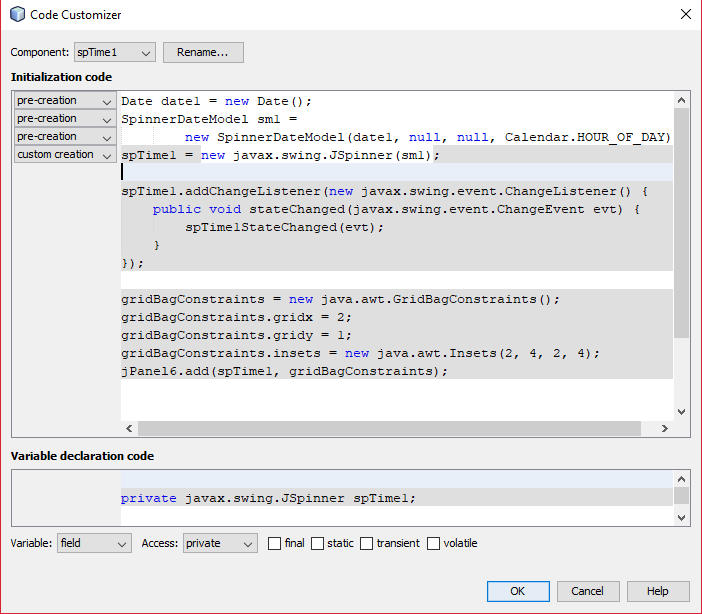
\includegraphics[width=0.70\textwidth]{Bilder/Java_Programm/SpinnerConfiguration}
  \end{center}
  \caption{Spinner Konfiguration}
  \label{SpinnerKonfiguration}
  \vspace{-70pt}
\end{wrapfigure}
\\ \\ In diesem Fenster ist der Code, welcher in den ersten vier Zeilen steht, hinzuzufügen. 
\\ Hier wird das Model für den Spinner gesetzt. Dieses Model gibt an, dass der Spinner ein Datum darstellen soll. Weiters wird nicht festgelegt was vom Datum angezeigt werden soll. Hier wird die Uhrzeit dargestellt. 
\\ \\ Diese Schritte sind für alle der vier verwendeten Spinner verwendet werden.

\vspace{60pt}

Zusätlich muss noch für jeden Spinner folgende Methode, im Constructor nach \textbf{initComponents();}, aufgerufen werden:
\begin{lstlisting}[style=Javastyle, caption=Spinner Zeitzone]
	JSpinner.DateEditor at1 = new JSpinner.DateEditor(spTime1, "HH:mm");
        	spTime1.setEditor(at1);
\end{lstlisting}

\vspace{10pt}

Im \textbf{Constructor} der \textbf{TimeManagement} Klasse werden, wenn das Fenster geöffnet wird, alle Spinner mit den momentanen Zeiten gefüllt. Zusätzlich werden noch die Häkchen, die festelegen ob eine Zeit aktiv ist, gesetzt.

\vspace{10pt}

Bevor das Fenster geschlossen wird, wenn \textbf{Abbrechen} gedrückt wird, wird überprüft, ob sich die Inhalte der Spinner veränder haben. Um dies zu überprüfen werden Events verwendet. Dafür wird für jeden Spinner das folgende Event verwendet:
\begin{lstlisting}[style=JavaStyle, caption=Spinner Event]
    private void spTime1StateChanged(javax.swing.event.ChangeEvent evt)                                     
    {                                         
        saved = false;
    }   
\end{lstlisting} 
Diese Event wird aufgerufen, wenn der Inhalt der Spinners verwendet wird. Dabei wird dann eine Boolean-Variable, die bekannt gibt, ob etwas verwendert wurde, auf \textbf{false} gesetzt. Wenn diese Boolean-Variable auf \textbf{false} ist, wird vor dem Beenden dem Benutzer eine Warnung ausgegeben, dass noch nicht gespeichert wurde. Zusätlich kann dann ausgwählt werden, ob wirklich ohne zu speichern beendet werden soll.
\\ \\ Wenn das Fenster mit \textbf{Ok} geschlossen wird, werden die Inhalte der Spinner, wenn sie geändert wurden, aus den Spinnern geholt. Zusätzlich wird das gleiche mit den ComboBoxes gemacht. Die Inhalte der Spinner und Comboxen werden anschließen in ein Dokument, also ein Format das für die Datenbank verständlich ist, gespeichert. Das Dokument sieht wie folgt aus:
\begin{lstlisting}[style=Javastyle, caption=Zeitendokument Getter-Methode]
// ... Code ...

newTimeDoc = new BasicDBObject("identifier", "Times")
                        .append("time1", time1)
                        .append("time1_active", time1_active)
                        .append("time2", time2)
                        .append("time2_active", time2_active)
                        .append("time3", time3)
                        .append("time3_active", time3_active)
                        .append("time4", time4)
                        .append("time4_active", time4_active);
\end{lstlisting}
Dieses Dokument wird anschließen mit folgender \textbf{Getter-Methode} geworfen damit sie in im \textbf{MainWindow} zugänglich ist:
\begin{lstlisting}[style=Javastyle, caption=Zeitendokument]
public BasicDBObject getNewTimeDoc()
    {
        return newTimeDoc;
    }
\end{lstlisting}

\newpage

\subsubsection{CreateUser}
\begin{wrapfigure}{l}{0.6\textwidth}
\vspace{-20pt}
  \begin{center}
    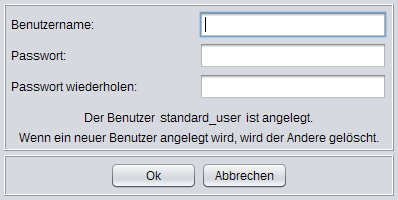
\includegraphics[width=0.60\textwidth]{Bilder/GUI/CreateUser}
  \end{center}
  \caption{CreateUser}
  \label{CreateUser}
  \vspace{-10pt}
\end{wrapfigure}
Die Klasse \textbf{CreateUser} bietet dem Benutzer die Möglichkeit einen Benutzer anzulegen. Mit dem angelegten Benutzer ist es möglich sich auf der Webseite der Anlage anzumelden. Die GUI ist in Abbildung \ref{CreateUser} zu sehen.
\\ Die GUI der Klasse ist ein Dialogfenster. Bei Dialogfenstern ist es üblich, dass sie mit \textbf{Ok} und \textbf{Abbrechen} bedienbar sind.
\\ \\ Es ist nur möglich einen Benutzer anzulegen. Wenn bereits ein Benutzer angelegt ist und dann ein Neuer angelegt wird, wird der alte Benutzer überschrieben. Um einen neuen Benutzer anzulegen müssen folgende Felder ausgefüllt werden: Benutzername, Passwort und Passwort wiederholen. Wenn eines dieser Felder leer gelassen wird, wird eine Fehlermeldung ausgegeben. Weiters wird eine Fehlermeldung ausgegeben, wenn die beiden Passwörter nicht übereinstimmen. Wenn alle drei Eingabefelder korrekt ausgefüllt wurden kann der Benutzer angelegt werden indem \textbf{Ok} gedrückt wird. Dadurch wird der Benutzer in das Programm übernommen und in die Datenbank gespeichert. Anschließend erscheint ein Informationsfenster welches den Benutzer darüber informiert, dass der Benutzer erfolgreich angelegt wurde. Danach schließt sich das Dialogfenster. Wenn anstatt von \textbf{Ok} \textbf{Abbrechen} gedrückt wird, schließt sich das Dialogfenster und die Änderungen werden verworfen.
\\ \\ Während das Dialogfenster geöffnet ist blockiert der ETD Thread an der Stelle, an der das Dialogfenster geöffnet wurde.

\vspace{10pt}

Um das Passwort einzugeben wird ein \textbf{PasswordField} verwendet. Diese Eingabefeld wird speziell dazu verwendet Passwörter einzugeben. Eine Besonderheit davon ist, dass die Passwörter nicht als Text sonder als Sternchen dargestellt werden. Eine weitere ist, dass der Inhalt eine Zeichenkette ist, also ein Feld von Characters: \textbf{char[]}. Weiters unterscheided sich auch das Abfragen des Inhaltes im Vergleich mit eienm normalen Textfeld. Beim \textbf{PasswordField} kann der Inhalt mit \textbf{passwordField.getPassword()} abgefragt werden.
\\ \\ Um das Password im Programm besser verarbeiten zu können wird es wie folgt in einen String umformatiert:
\begin{lstlisting}[style=Javastyle, caption=char zu String]
	String string_password = valueOf(char_password);
\end{lstlisting}

\vspace{10pt}

Um eine gewisse Sicherheit zu gewährleisten wird das Password, bevor es in der Datenbank gespeichert wird, gehasht. Um das Password zu hashen wird der \textbf{SHA-512} verwendet. Im Programm wird das Passwort nur einmal gehasht. Falls die Katzenfütterungsanlage in Serie gehen sollte, sollte das Passwort öfters gehasht werden um die Sicherheit zu erhöhen.
\\ Das Password wurde wie folgt gehasht:
\begin{lstlisting}[style=Javastyle, caption=Hash Passwort]
	public static String hash(String passwordToHash, String salt)
    {
        String generatedPassword = null;
        try
        {
            MessageDigest md = MessageDigest.getInstance("SHA-512");
            md.update(salt.getBytes("UTF-8"));
            byte[] bytes = md.digest(passwordToHash.getBytes(StandardCharsets.UTF_8));
            StringBuilder sb = new StringBuilder();
            for (int i = 0;
                    i < bytes.length;
                    i++)
            {
                sb.append(Integer.toString((bytes[i] & 0xff) + 0x100, 16).substring(1));
            }
            generatedPassword = sb.toString();
        }
        catch (NoSuchAlgorithmException e)
        {
            e.printStackTrace();
        }
        catch (UnsupportedEncodingException ex)
        {
            Logger.getLogger(HashPassword.class.getName()).log(Level.SEVERE, null, ex);
        }
        return generatedPassword;
    }
\end{lstlisting}
Mit dem Parameter \textbf{String salt} kann noch ein String übergeben werden welcher vor dem Hashen des Passworts am Passwort angehänt wird. Somit wird die Entschlüsselung des Passwort nochmals erschwert und die Sicherheit erhöht sich.

\vspace{10pt}

Bevor das Fenster geschlossen wird, wenn \textbf{Update} gedrückt wird, wird überprüft, ob sich die Inhalte der Text- und Passwortfelder verändert haben. Dabei wird vom Event überwacht, ob in dem Feld ein neues Zeichen eingegeben wird. Danach wird eine Boolean-Variable, die angibt ob gespeichert wurde, auf \textbf{false} gesetzt. Das Event für das Textfeld sieht wie folgt aus:
\begin{lstlisting}[style=Javastyle, caption=Textfeld Event]
private void tfUser_nameKeyPressed(java.awt.event.KeyEvent evt)                                       
    {                                           
        saved = false;
    }
\end{lstlisting}
Wenn die Variable \textbf{false} ist, also noch nicht gespeichert wurde, wird dem Benutzer die Warnung ausgegeben werden, dass die veränderten Daten noch nicht gespeichert sind.

\vspace{10pt}

Wenn das Dialogfenster mit \textbf{Ok} bestätigt wird, wird das Benutzername und das Passwort in ein Dokument, welches für die Datenbank verständlich ist, gespeichert. Dieses Dokument sieht wie folgt aus:
\begin{lstlisting}[style=Javastyle, caption=Benutzerdokument]
newUserDoc = new BasicDBObject("identifier", "User").append("user_name", 
	user_name).append("user_password", hashedPassword);
\end{lstlisting}

Dieses Dokument wird anschließend noch mit einer \textbf{Getter-Methode} geworfen damit es im \textbf{MainWindow} zugägnlich ist:
\begin{lstlisting}[style=Javastyle, caption=Benutzerdokument Getter-Methode]
public BasicDBObject getNewUserDoc()
    {
        return newUserDoc;
    }
\end{lstlisting}

\subsubsection{ManualControl}
  \begin{figure}[H]
    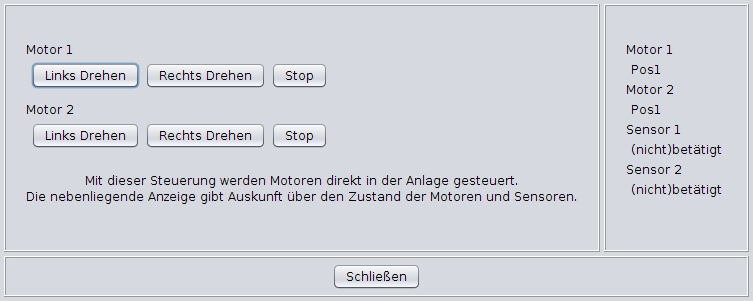
\includegraphics[width=0.90\textwidth]{Bilder/GUI/ManualControl}
    \caption{ManualControl}
  \label{ManualControl}
  \end{figure}
In der Klasse \textbf{ManualControl} wird eine manuelle Steuerung für die Motoren implementiert. Dies erleichtert dem Benutzer das Reinigen der Anlage, weil er zum Beispiel die Drehplatte, mit den Futterschüsseln, immer nachdrehen kann. Das gleiche gilt für das Förderband.
\\ Die GUI ist in Abbildung \ref{ManualControl} zu sehen.
\\ Die GUI der Klasse ist ein Steuerfenster. Da dieses Fenster ein Steuer- und kein Dialogfenster ist, werden kein \textbf{Ok} und \textbf{Abbrechen} benötigt. Aus diesem Grund ist nur ein Knopf \textbf{Schließen} vorhanden.

\vspace{10pt}

Wie beim Dialogfenster blockiert das Steuerfenster den EDT der Stelle wo es geöffnet wurde bis es wieder geschlossen wurde.

\vspace{10pt}

Dieses Fenster ist aus Sicherheitsgründen nur dann aufrufbar, wenn der Maschinenzustand auf Aus ist. Der Grund dafür ist, dass es zu Fehlern kommen kann, wenn während einer Fütterung ein Motor ein oder aus geschalten wird.
\\ Weiters wird der Benutzer bevor er dieses Steuerfenster öffnet darüber infomiert, dass er nun direkt die Motoren steurt. Zusätlich wird der Benutzer gefragt ob er die Steuerung wirklick öffnen will.
\\ Der Benutzer kann nun beide Motoren unabhäging voneinander steuern. Er kann die Motoren in und gegen den Uhrzeigersinn drehen. Dazu muss er den Knopf mit der jeweiligen Drehrichtung im Steuerungsfenster klicken. Die Motoren sind mit dem jeweiligen Stop-Knopf wieder stopbar.
\\ Falls die Motoren vom Benutzer vor dem Schließen des Fensters nicht gestoppt werden, werden diese automatisch vom Programm gestopt. Dies dient dazu, dass sichergestellt ist, dass die Motoren immer gestopt werden.
\\ Die Methode zum Schließen des Fensters, welche auch die Motoren stopt, sieht wie folgt aus:
\begin{lstlisting}[style=JavaStyle, caption=Motoren stoppen und Fenster schließen]
	private void onSchließen(java.awt.event.ActionEvent evt)                                
    	{                                 
       		// stop engines when closing the conrtol dialog - security measurement
        	pi4j_instance.stopEngine1();
        	pi4j_instance.stopEngine2();
        
        	dispose();
    	} 
\end{lstlisting}

\vspace{10pt}

Neben dem Bereich für die Steuerung befindet sich noch ein Bereich in dem die Echtzeit-Zustände aller Motoren und Sensoren angezeigt werden. So kann der Benutzer ohne in die Anlage zu sehen feststellen, ob sich ein Motor dreht oder ein Sensor betätigt ist.

\vspace{10pt}

Die Motoren werden gesteuert, indem beim Drücken eines Knopfes, eine Methode aus dem \textbf{pi4j Singleton} (Kaptiel \ref{subsec:pi4j}) aufgerufen wird. Aus dieser Klasse ausgehend werden die Output-Pins und in weiterer Folge die Motoren gesteuert.
\\ Wenn ein Knopf gedrückt wird, wird die jeweilige zum Knopf gehörente Methode aufgerufen. Dies kann wie folt aussehen:
\begin{lstlisting}[style=JavaStyle, caption=Motoren drehen] 
	private void onMoveEngine1Counterclockwise(java.awt.event.ActionEvent evt)                                               
    	{                                                   
        	pi4j_instance.moveEngine1Counterclockwise();
    	}  
\end{lstlisting}

\vspace{10pt}

Um die aktuellen Positionen der Motoren und Zustände der Sensoren zu ermitteln und ausgeben wird ein SwingWorker verwendet. Dies ist unter Kapitel \ref{subsubsec:Positionsinformation} genauer beschrieben

\newpage

\subsubsection{Positionsinformation} \label{subsubsec:Positionsinformation}
\begin{wrapfigure}{l}{0.3\textwidth}
\vspace{-20pt}
  \begin{center}
    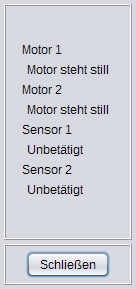
\includegraphics[width=0.30\textwidth]{Bilder/GUI/Positionsinformation}
  \end{center}
  \caption{Positionsinformation}
  \label{Positionsinformation}
  \vspace{-10pt}
\end{wrapfigure}
text

\newpage

\subsubsection{SystemInfo}
bild fehlt weil server nicht gelaufen ist

\newpage

\subsubsection{Update}\label{subsubsec:Update}
\begin{wrapfigure}{l}{0.4\textwidth}
\vspace{-20pt}
  \begin{center}
    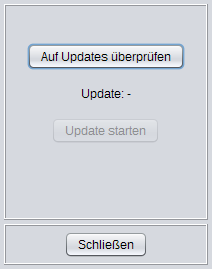
\includegraphics[width=0.40\textwidth]{Bilder/GUI/Update1}
  \end{center}
  \caption{Update1}
  \label{Update}
  \vspace{-10pt}
\end{wrapfigure}
text

\begin{wrapfigure}{l}{0.4\textwidth}
\vspace{-20pt}
  \begin{center}
    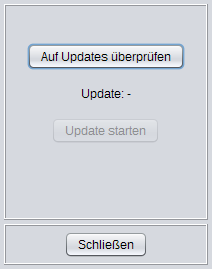
\includegraphics[width=0.40\textwidth]{Bilder/GUI/Update1}
  \end{center}
  \caption{Update1}
  \label{Update}
  \vspace{-10pt}
\end{wrapfigure}
text

\section{Zusammenfassung/Verbesserungsmöglichkeiten}
\subsection{Probleme mit Mongodb am Raspberry}
\subsection{Probleme mit pi4j -> Snapshotversion verwendet - ansonsten werden pins nicht erkannt}
\subsection{GUI auf "Touchscreen-Design" abändern}
\subsection{Besser Benutzerverwaltung - Mehrere Benutzer anlegen}
\subsection{Selbst erstellbare Vorlagen in denen Zeiten gespeichert werden}
